\chapter{Requirements Engineering}
\label{sec:reqeng}

In this chapter, we consider the requirements engineering (RE) activities for the design of CPSs. Specifically, we consider the specification and documentation of requirements placed upon a CPS. These requirements may, for example, impose restrictions, define system capabilities or identify qualities of a system. The requirements should indicate some value or use for the different stockholders of a CPS.

As described in the previous chapter, traceability needs requirements to be defined as early as possible in a development process, and these must be recorded in Modelio for the machine-assisted traceability information to be recorded accurately. It is therefore appropriate to consider requirements processes for such developments at this stage.

In this remainder of this chapter, we discuss the needs for requirements engineering in CPS development, in particular based on the experience of the industrial partners for INTO-CPS. We describe one possible approach to RE for CPS, specifically adapting the SoS-ACRE approach for systems-of-systems (SoSs) to CPS. Note however that this approach is not mandatory, and in general RE processes and tools vary widely across organisations and domains. For this reason, tool support for traceability in INTO-CPS begins once requirements have been defined and can be added to Modelio. The diagrams described in the example are not part of INTO-CPS SysML specification. Therefore, this chapter should truly be treated as guidance, primarily serving to highlight the nature of RE for CPS, which may be of use for both new and more experienced CPS teams.

%In this project, we consider the state in the art of RE in both CPS and Systems of Systems (SoSs), reusing a previously defined approach to RE as applicable.

\section{Requirements Engineering and Cyber-Physical Systems}

The main issue of concern for RE in CPSs is that of differing domain contexts~\cite{Wiesner&14}. In addition, it has been noted that there are overlaps in challenges in CPSs and SoSs~\cite{Penzenstadler&12}--- especially independence, evolution and, increasingly, distribution. As described by Lewis et al.~\cite{Lewis&09}, as system architectures become more complex, there is often a need to consider requirements and structural architectures during the RE process. The authors suggest that an engineer should identify the system needs, component interactions and stakeholders, and map those needs onto those interested parties. %In Deliverable D3.1b~\cite{INTOCPSD31b}, we also surveyed several projects that had RE as a focus, or part of their focus.

As research in RE in CPS is a nascent field, we suggest one approach is to adopt RE processes from the SoS world, rather than defining an approach specifically for CPSs.  In chapter, we consider SoS-ACRE (System of Systems Approach to Context-based Requirements Engineering)~\cite{Holt&15}, as an example. This approach was adapted from standard systems engineering, and tailored for SoSs--- enabling the identification and reasoning about requirements across constituent systems of an SoS and understanding multi-stakeholder contexts. We suggest it might be useful to organisations trying to approach RE for CPS.

\section*{INTO-CPS industry partners and RE}

At the beginning of the INTO-CPS project, the four industrial partners were surveyed about their use of various technologies and methods, including requirements engineering~\cite{INTOCPSD31b}. Microsoft Excel was quoted as being used by three partners (UTRC, TWT and CLE), IBM Rational Doors used by one partner (UTRC), and Microsoft Word by one partner (AI).

Issues raised by industrial partners include:
\begin{itemize}
  \item Language/terminology of the requirements not consistent;
  \item Different people involved in the workflow do not have common understandings of requirements;
  \item Requirements traceability is considered to be highly inefficient and time consuming;
  \item Different people have to meet together and generate proofs among each other to validate dependable requirements; and
  \item Stakeholders do not have a clear vision about the product and tend to disagree on the objectives.
\end{itemize}

As can be seen, the above issues may be due to not having a rigorous RE approach, but also due to the challenges in CPSs--- that of different domains. In this section, we consider how a context-based approach to RE (SoS-ACRE) may be incorporated into the INTO-CPS tool chain, in particular using both the INTO-CPS technologies and the industrial partners' baseline technologies.

%%\fbox{check other sources for use on Excel in industry -- are industrial partners typical?}


\section{The SoS-ACRE View of Requirements}

We first consider the collection of views defined in SoS-ACRE, and their applicability to CPS engineering and the INTO-CPS tool chain. These views could be represented as diagrams in SysML\footnote{Note that SoS-ACRE is not specifically supported as a Modelio plug-in, but other equivalent diagrams could be used.}, or as we describe, could equally be represented in other tools where these are already used (e.g. Excel). Examples of each view are shown in Figures~\ref{fig:re-singlesysml}, \ref{fig:re-multisysml}, \ref{fig:re-uri-excel-sysml} and \ref{fig:re-excel-sysml}. %using  technologies relevant to INTO-CPS.

%\fbox{include example figures?}

\begin{description}
\item[Source Element View (SEV)] The SEV defines a collection of source materials from which requirements are derived. In SoS-ACRE, a SysML block definition diagram is considered. In INTO-CPS, this view could also be represented using an Excel table or Word document (with each source having a unique identifier), or by simply referring to source documents using OSLC traces.

\item[Requirement Description View (RDV)] The RDV is used to define the requirements of a system and forms the core of the requirement definition. SoS-ACRE suggests the use of SysML requirements diagram or in tabulated form, such as through the use of Excel. In addition, specifying requirements in  Doors would  support this view.

\item[Context Definition View (CDV)] The CDV is a useful view for CPS engineering in order to explicitly identify interested stakeholders and points of context in the system development, including customers, suppliers and system engineers themselves. In SoS-ACRE, they are defined using SysML block definition diagrams, and could also be represented using an Excel table or Word document (with each context having a unique identifier). This diagram type could be useful when identifying the divide in CT/DE and cyber-physical elements of a system.

\item[Requirement Context View (RCV)] In SoS-ACRE, a RCV is defined for each constituent system context identified in CDVs. This is appropriate when there is a set of diverse system owners, which is typical for SoSs and increasingly CPSs. A \textbf{Context Interaction View (CIV)} is then defined to understand the overlap of contexts and any common/conflicted views on requirements. In a CPS, however, there may not be such a clear delineation between the owners of constituent  system components. However, if we consider the different domains (e.g. CT/DE or cyber/physical divides) as different contexts, then this approach would be useful. In SoS-ACRE, RCVs and CIVs are both defined with SysML use case diagrams. Excel could be used if unique identifiers are defined for contexts and requirements as described earlier.

\item[Validation View (VV)] VVs, defined as SysML sequence diagrams in SoS-ACRE, describe validation scenarios for a SoS to ensure each constituent system context understands the correct role of the requirements in the full SoS. This is not an obvious fit in CPS engineering, and therefore not necessarily required.

\end{description}

\section{The SoS-ACRE RE Process}

The SoS-ACRE requirement engineering process may be useful for organisations wishing to better understand requirements for CPSm, particularly across multiple domains. It is a lightweight process, and therefore suitable for small- to medium-sized enterprises. Organisations with established may not feel the need to radically alter their existing practice, but may find it instructive to consider how their current processes might be updated or revised to consider better CPS requirements.

% The requirements management is considered to be too heavyweight a target for translation. This is largely due to the fact that we are currently less concerned with requirement change/different processes.

A SoS-ACRE process for CPS should include the following steps:

\begin{enumerate}
\item Identify and record source elements. This would be using a SEV, or simply recording paths to relevant files or documents.

\item Record system-level functional and non-functional requirements. Requirements may be derived using RDVs, and we could consider domain-specific requirements (e.g. cyber or physical), or analysis-specific requirement types (e.g. DSE or testing requirements).

\item Model initial System structure using INTO-CPS ASD. This will identify the cyber and physical elements and the domain/phenomena of the CPS. This may also give initial idea of component functionalities, which may lead to a repeat of Step 2 above\footnote{In the process of architectural modelling, it may also be necessary to redefine contexts depending on whether different simulation tools, or indeed different components of a model, are better able to provide the requirements of the CPS.}.

\item Define the various contexts in CDVs -- both external stakeholders, and if appropriate, contexts for the different components. If only a single system context is defined, then a single RCV is defined. However, if multiple contexts are defined for a CPS, then several RCVs are to be defined, along with a CIV to explore requirements from multiple contexts.

\item Trace the requirements through INTO-CPS tool chain models and results. This was covered in the previous chapter, however we revisit it below in the context of requirements.
\end{enumerate}

\section{Using technologies with SoS-ACRE}

%In this final section, we consider initial approaches to realise the relevant SoS-ACRE views using the INTO-CPS technologies and those used by industrial partners. This is not expected to constitute final guidelines on this area, as we would make use of INTO-CPS technology currently in development -- namely traceability and provenance support.

As INTO-CPS does not specifically support SoS-ACRE. Indeed INTO-CPS does not mandate and specific approach to RE, because of the wide variety of approaches in industry. We conclude this chapter with an example of how a SoS-ACRE (or other RE process) could be integrated into an INTO-CPS development. We describe a range of permutations of the use of models and documents for recording the requirements engineering process described above. In addition, we include discussions on the links between requirements and architectural models--- identified above as a key method for requirements engineering in CPSs. %We also refer to OSLC and Prov links, which could be linked into the INTO-CPS traceability, though are not supported by the tool chain at the end of the project. Further information on OSLC can be found in Deliverable D3.3b~\cite{INTOCPSD3.3b}.

\begin{description}

\item[URI, Excel and SysML]

We first consider an approach using URIs for the source elements, an Excel document (or a collection of Excel tables) for the RDV, CDV, RCV and CIV of SoS-ACRE. A SysML model in Modelio can be used to define the architecture of the multi-model. Internal tracing in Excel can be achieved using identifiers referenced between sheets. Excel requirements can be replicated in Modelio then traced to elements in the INTO-CPS tool chain automatically. Figure~\ref{fig:re-uri-excel-sysml} presents an example with URI, Excel and SysML models and OSLC links between the artefacts.

\item[Excel and SysML]

The next approach uses Excel to define the SEV and RDV of SoS-ACRE, a SysML model to define the context-oriented views (CDV, RCV and CIV) and a separate architectural model to define the CPS architecture. The Excel requirements can then be mirrored in a Modelio model, and linked to the architectural model. The INTO-CPS traceability features can trace the requirement artefacts to the architectural model. Additional OSLC links could be added manually to link elements of the Excel requirements and context views in a SysML.  Figure~\ref{fig:re-excel-sysml} presents an example with URI, Excel and two SysML models with OSLC links between the artefacts.

\item[Single SysML model]

The next permutation is to use a single SysML model for both requirements engineering and architectural modelling. Such a model will contain all SoS-ACRE views\footnote{Note that Modelio does not currently provide an extension for SoS-ACRE, but these views can be realised using existing SysML stereotypes.} (SEV, RDV, CDV, RCV and CIV), in addition to diagrams defined using the INTO-CPS profile for the CPS composition and connections. Modelling in this way enables trace links to be defined inside a single SysML model. Figure~\ref{fig:re-singlesysml} presents an example SysML model with trace relationships.



\item[SysML requirements and SysML architectural models]

The final permutation is to use SysML for both requirements engineering and architectural modelling, however to use two separate models for the two activities (one containing the RE views (SEV, RDV, CDV, RCV and CIV) and another for architectural diagrams (ASD and CD)). We consider this permutation with two SysML models in addition to the single SysML model, because the requirements engineering and architectural modelling activities are often considered separately, with different engineering teams comprised of engineers with specialist skills. As such we can assume there are cases where these teams have ownership of different models.
Trace links may be used within each individual model (for example, tracing from source elements to requirements in a RE model), and OSLC links defined to trace between requirements elements and architectural elements. Figure~\ref{fig:re-multisysml} presents an example with two SysML models with trace relationships and OSLC links between the models.

\begin{figure}
	\centering
	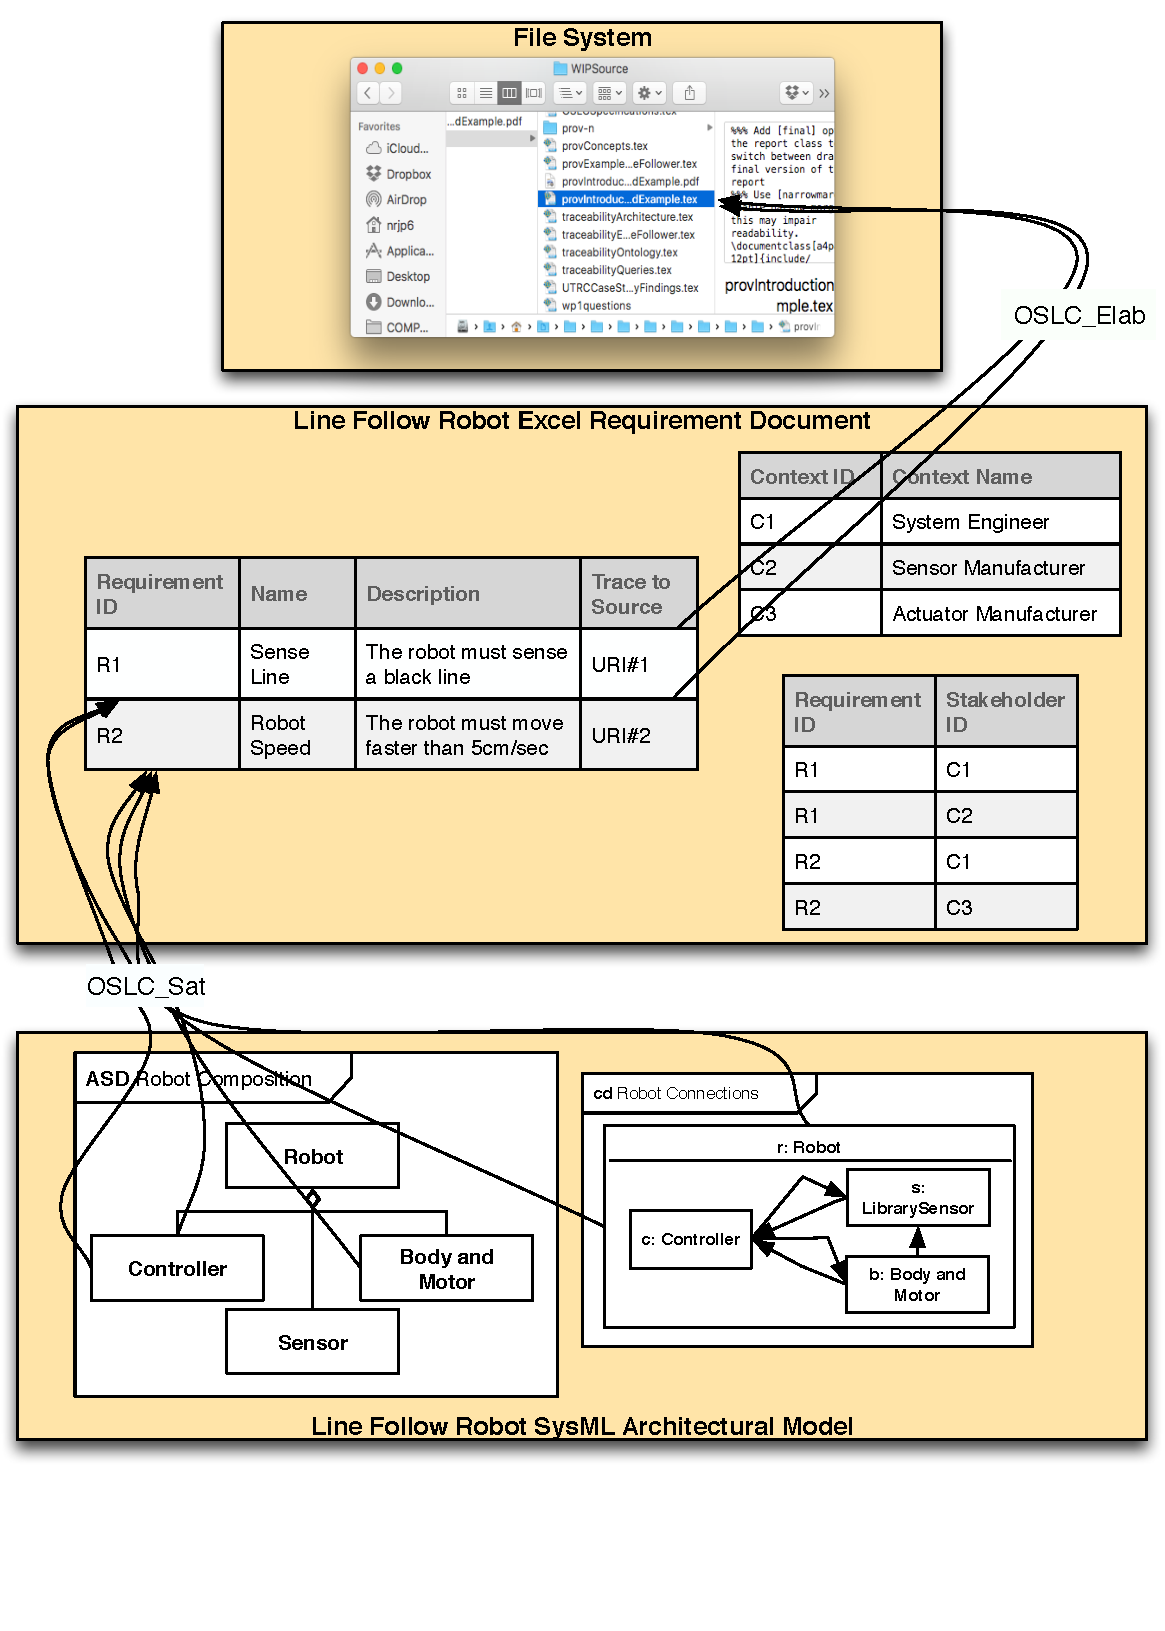
\includegraphics[scale=0.65]{figures/RE_3}
\caption{URI, Excel and SysML -- model overview}
\label{fig:re-uri-excel-sysml}
\end{figure}

\begin{figure}
	\centering
	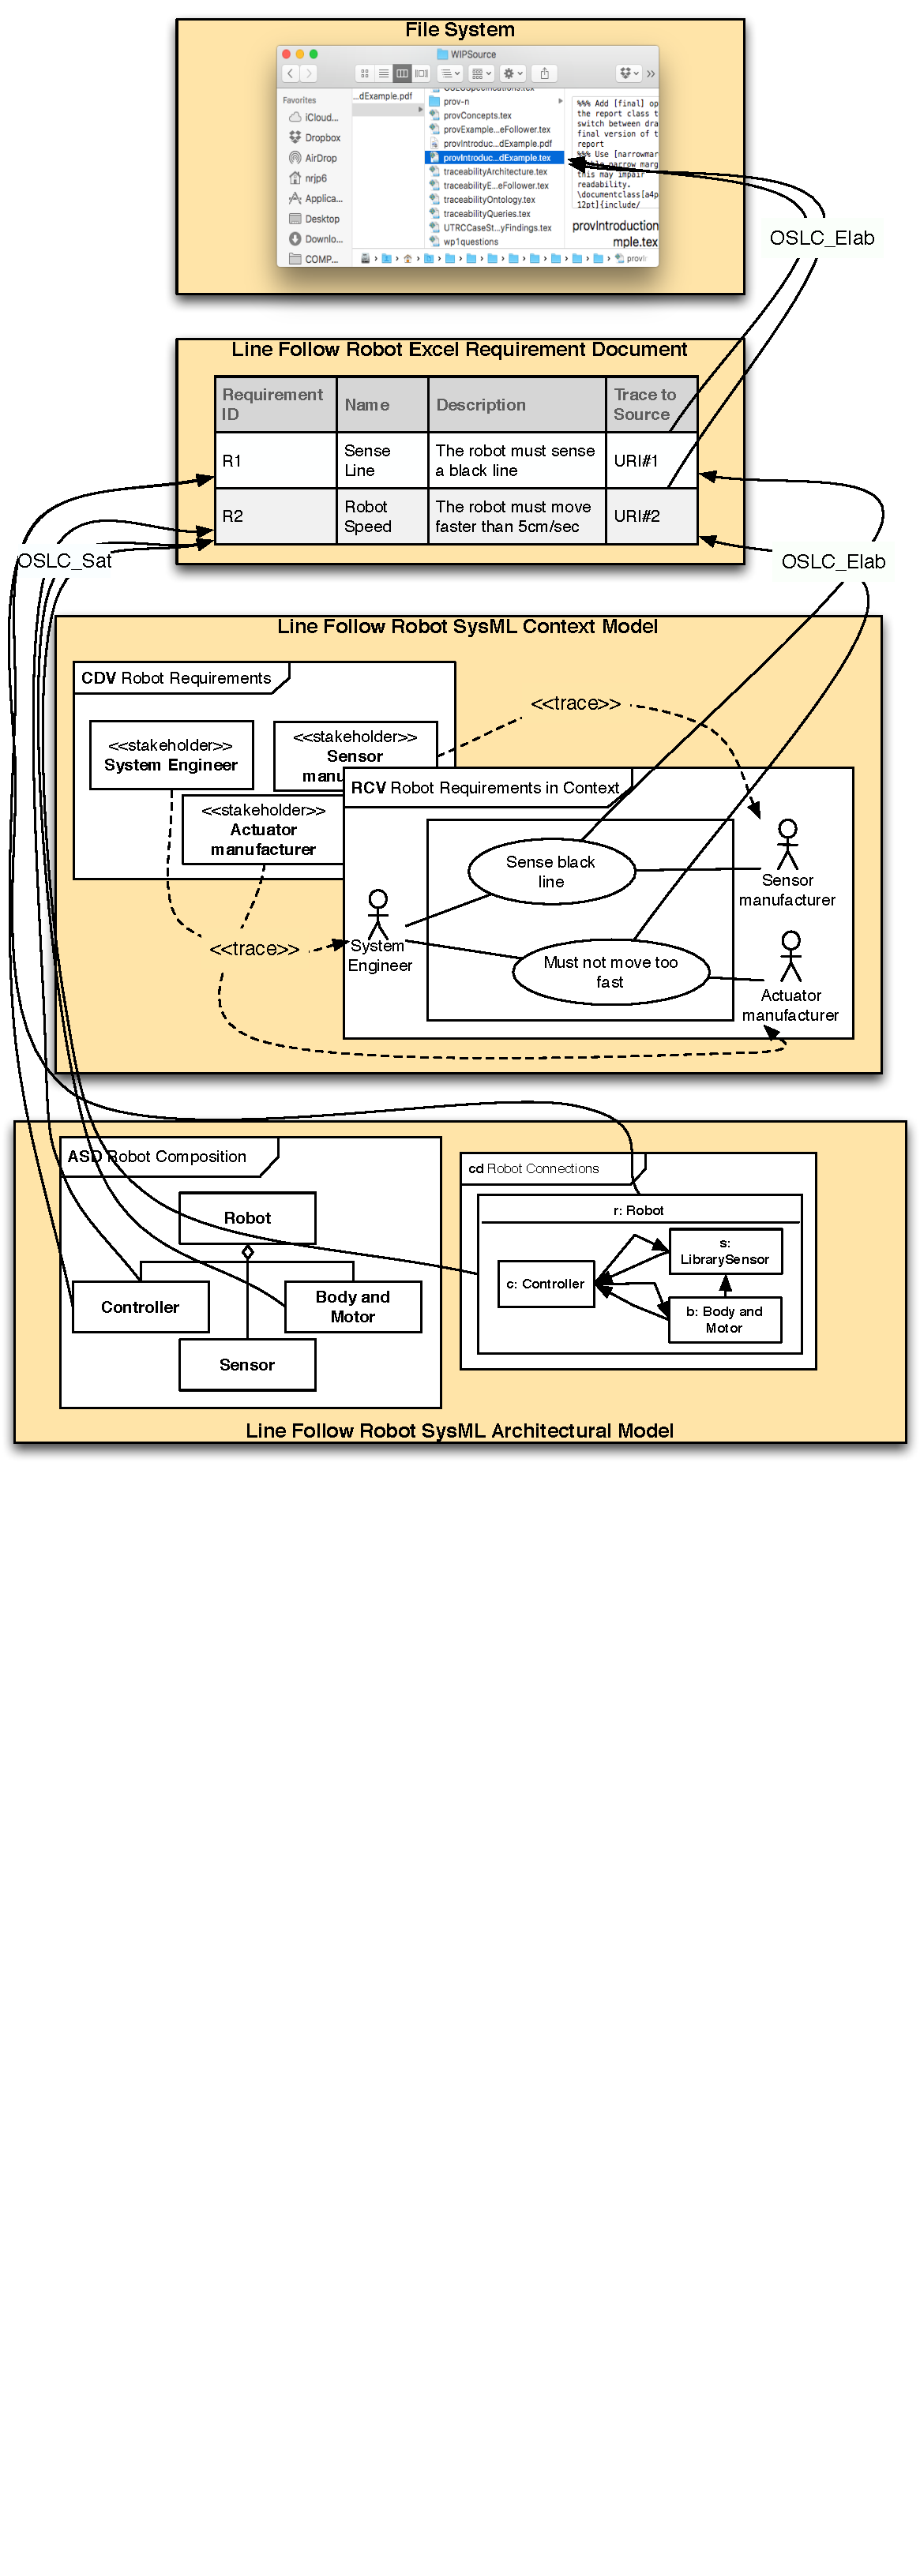
\includegraphics[width=0.8\textwidth]{figures/RE_4}
\caption{Excel and SysML -- model overview}
\label{fig:re-excel-sysml}
\end{figure}

\begin{figure}
	\centering
	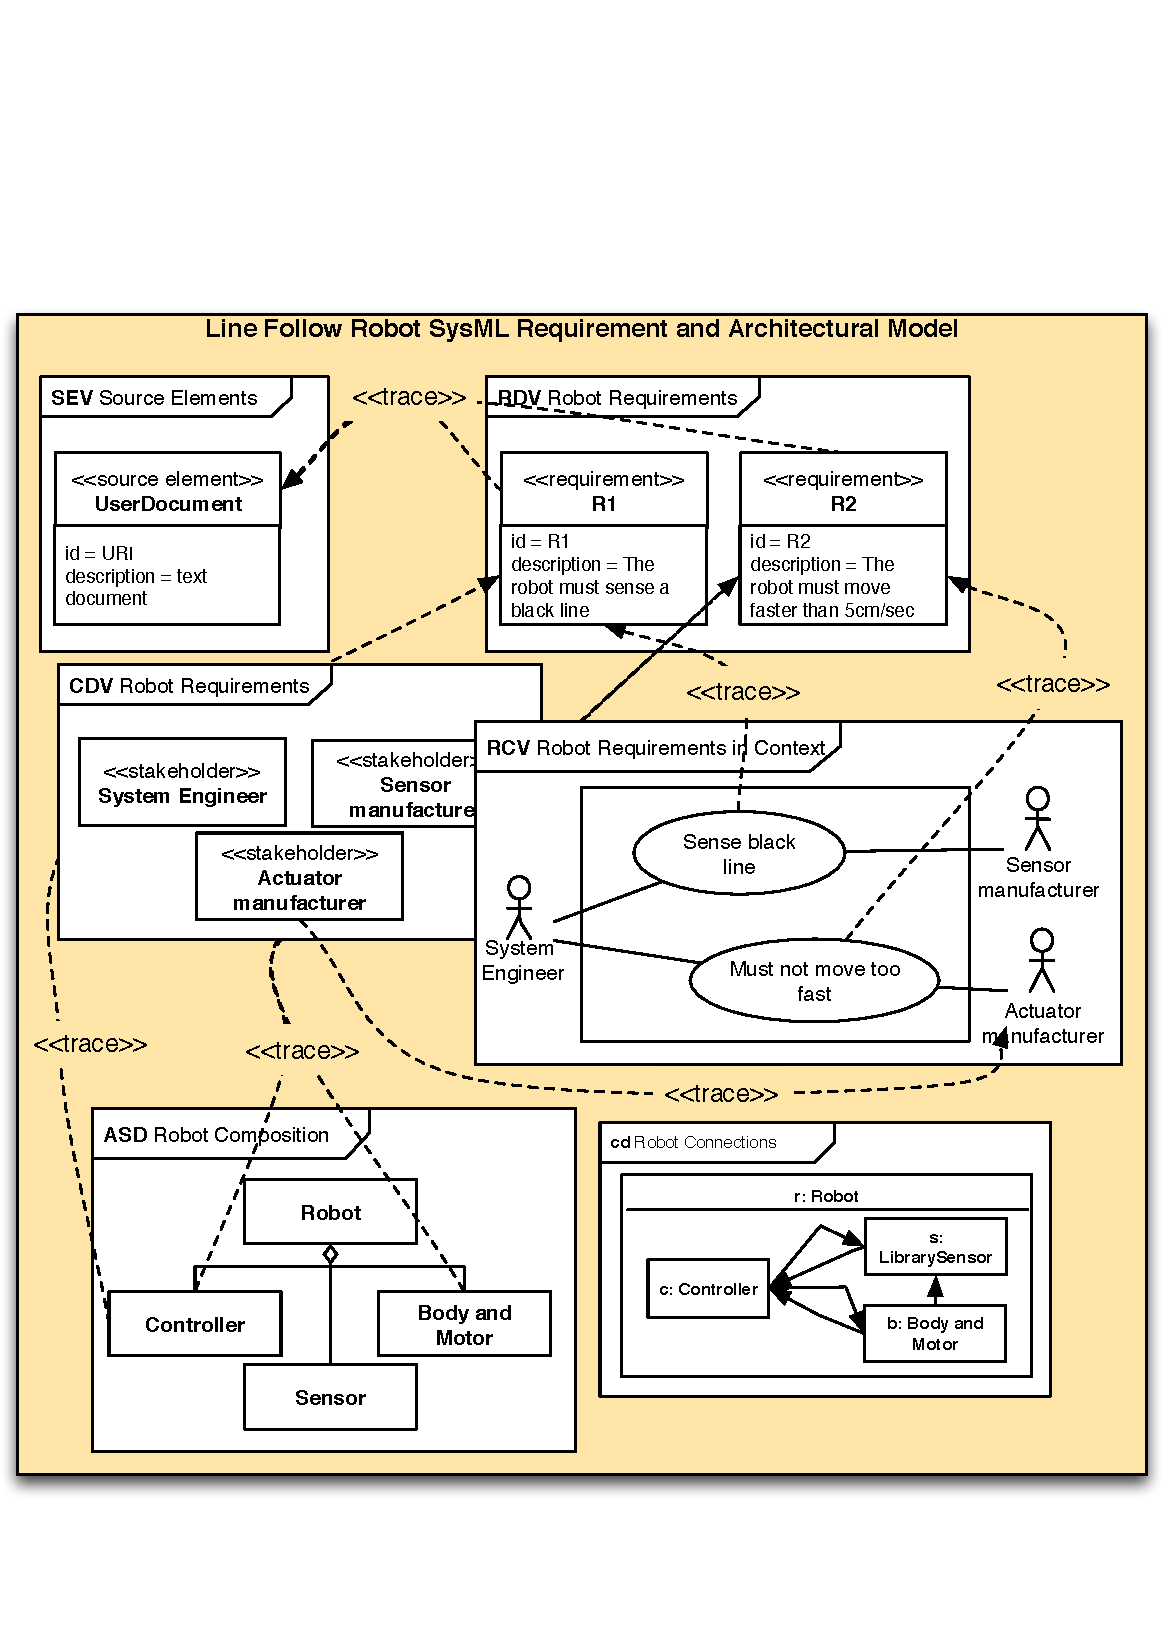
\includegraphics[scale=0.7]{figures/RE_1}
\caption{Single SysML model -- model overview}
\label{fig:re-singlesysml}
\end{figure}

\begin{figure}
	\centering
	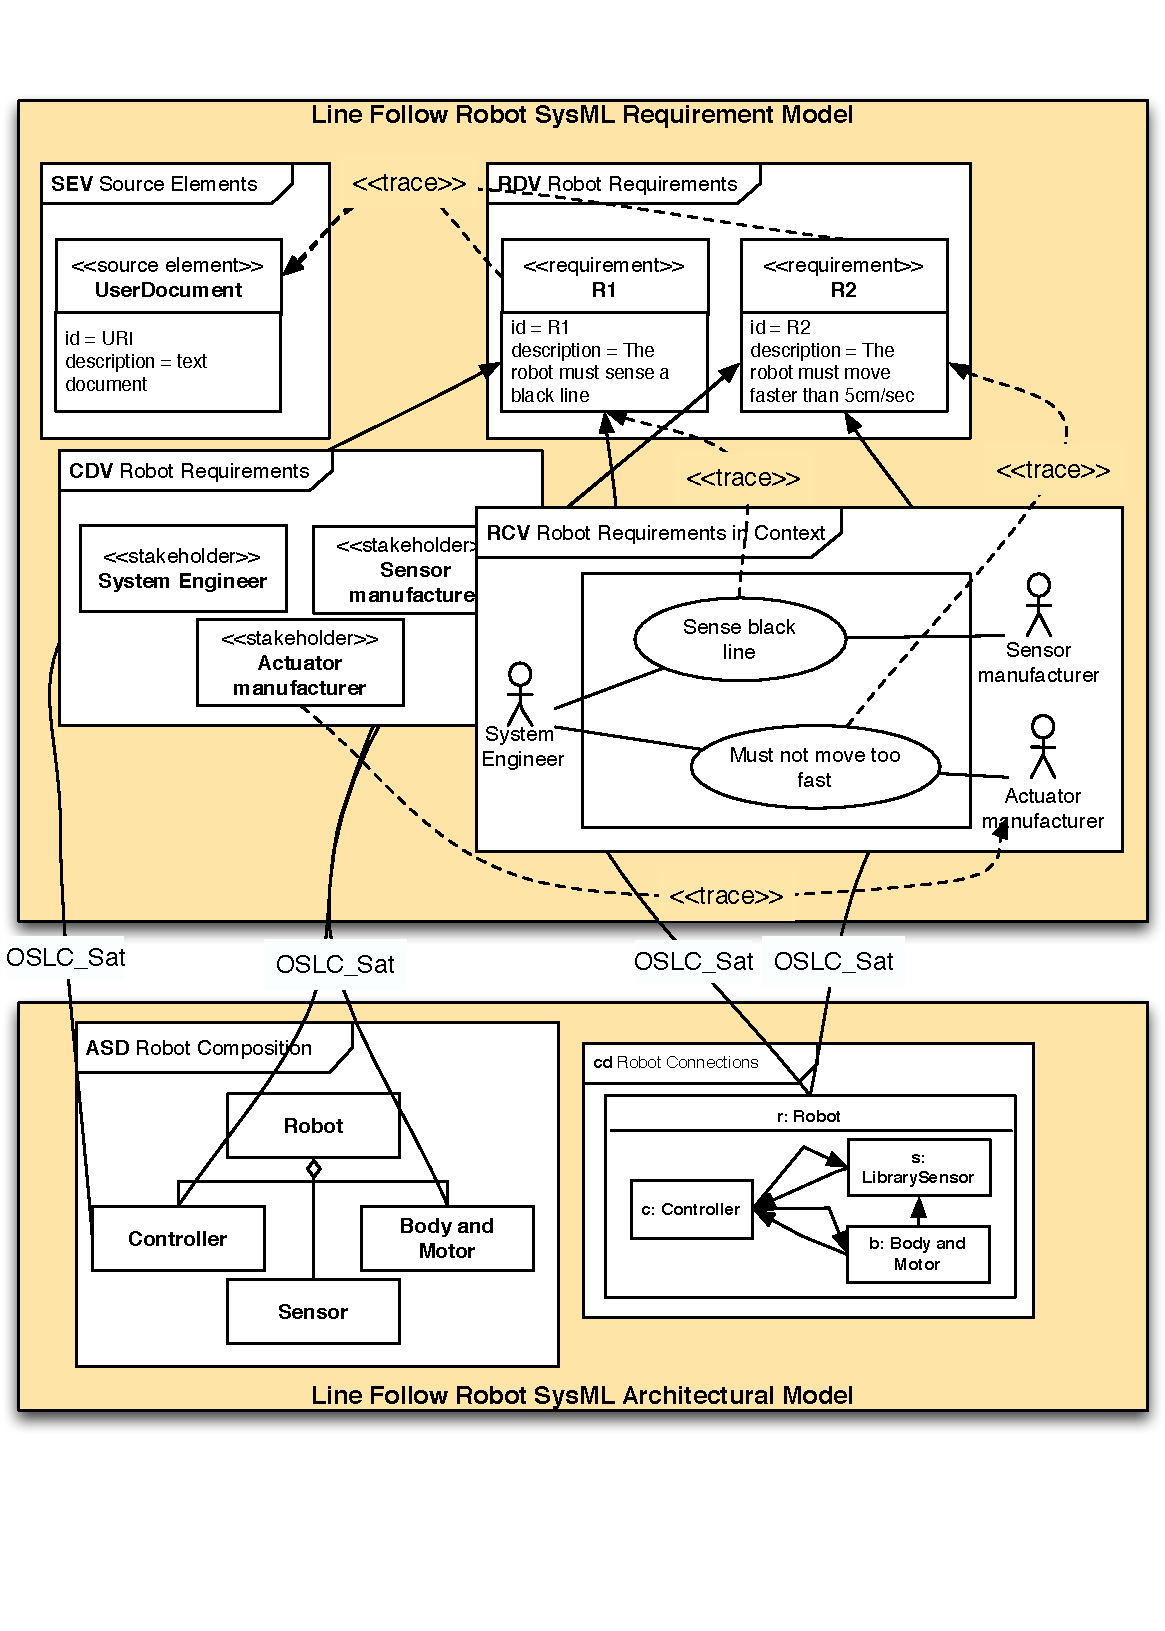
\includegraphics[scale=0.7]{figures/RE_2}
\caption{SysML requirements and SysML architectural models -- model overview}
\label{fig:re-multisysml}
\end{figure}
\end{description}

%
% MOVED TO FINAL CHAPTER
%

%\section{Future Guidelines}
%
%In the final year of the INTO-CPS project, we will consider additional guidelines in RE--- specifically regarding links from requirements to modelling for analysis  and to the analysis results themselves. For example, we would consider guidelines for specifying requirements that influence objectives defined in design space exploration. This is alluded to in Section~\ref{sec:dse-linefollow}. We shall also consider how this relates to co-simulation and the existing work in test automation -- as reported in Deliverable D5.1b~\cite{INTOCPSD51b}.
